\documentclass[spec, och, labwork]{shiza}
% параметр - тип обучения - одно из значений:
%    spec     - специальность
%    bachelor - бакалавриат (по умолчанию)
%    master   - магистратура
% параметр - форма обучения - одно из значений:
%    och   - очное (по умолчанию)
%    zaoch - заочное
% параметр - тип работы - одно из значений:
%    referat    - реферат
%    coursework - курсовая работа (по умолчанию)
%    diploma    - дипломная работа
%    pract      - отчет по практике
% параметр - включение шрифта
%    times    - включение шрифта Times New Roman (если установлен)
%               по умолчанию выключен
\usepackage{subfigure}
\usepackage{tikz,pgfplots}
\pgfplotsset{compat=1.5}
\usepackage{float}

%\usepackage{titlesec}
\setcounter{secnumdepth}{4}
%\titleformat{\paragraph}
%{\normalfont\normalsize}{\theparagraph}{1em}{}
%\titlespacing*{\paragraph}
%{35.5pt}{3.25ex plus 1ex minus .2ex}{1.5ex plus .2ex}

\titleformat{\paragraph}[block]
{\hspace{1.25cm}\normalfont}
{\theparagraph}{1ex}{}
\titlespacing{\paragraph}
{0cm}{2ex plus 1ex minus .2ex}{.4ex plus.2ex}

% --------------------------------------------------------------------------%


\usepackage[T2A]{fontenc}
\usepackage[utf8]{inputenc}
\usepackage{graphicx}
\graphicspath{ {./images/} }
\usepackage{tempora}

\usepackage[sort,compress]{cite}
\usepackage{amsmath}
\usepackage{amssymb}
\usepackage{amsthm}
\usepackage{fancyvrb}
\usepackage{listings}
\usepackage{listingsutf8}
\usepackage{longtable}
\usepackage{array}
\usepackage[english,russian]{babel}

% \usepackage[colorlinks=true]{hyperref}
\usepackage{url}

\usepackage{underscore}
\usepackage{setspace}
\usepackage{indentfirst} 
\usepackage{mathtools}
\usepackage{amsfonts}
\usepackage{enumitem}
\usepackage{tikz}
\usepackage{minted}

\newcommand{\eqdef}{\stackrel {\rm def}{=}}
\newcommand{\specialcell}[2][c]{%
\begin{tabular}[#1]{@{}c@{}}#2\end{tabular}}

\renewcommand\theFancyVerbLine{\small\arabic{FancyVerbLine}}

\newtheorem{lem}{Лемма}

\begin{document}

% Кафедра (в родительном падеже)
\chair{}

% Тема работы
\title{Задача о самом длинном простом цикле}

% Курс
\course{3}

% Группа
\group{331}

% Факультет (в родительном падеже) (по умолчанию "факультета КНиИТ")
\department{факультета КНиИТ}

% Специальность/направление код - наименование
%\napravlenie{09.03.04 "--- Программная инженерия}
%\napravlenie{010500 "--- Математическое обеспечение и администрирование информационных систем}
%\napravlenie{230100 "--- Информатика и вычислительная техника}
%\napravlenie{231000 "--- Программная инженерия}
\napravlenie{100501 "--- Компьютерная безопасность}

% Для студентки. Для работы студента следующая команда не нужна.
% \studenttitle{Студентки}

% Фамилия, имя, отчество в родительном падеже
\author{Окунькова Сергея Викторовича}

% Заведующий кафедрой
% \chtitle{} % степень, звание
% \chname{}

%Научный руководитель (для реферата преподаватель проверяющий работу)
\satitle{доцент} %должность, степень, звание
\saname{А. Н. Гамова}

% Руководитель практики от организации (только для практики,
% для остальных типов работ не используется)
% \patitle{к.ф.-м.н.}
% \paname{С.~В.~Миронов}

% Семестр (только для практики, для остальных
% типов работ не используется)
%\term{8}

% Наименование практики (только для практики, для остальных
% типов работ не используется)
%\practtype{преддипломная}

% Продолжительность практики (количество недель) (только для практики,
% для остальных типов работ не используется)
%\duration{4}

% Даты начала и окончания практики (только для практики, для остальных
% типов работ не используется)
%\practStart{30.04.2019}
%\practFinish{27.05.2019}

% Год выполнения отчета
\date{2022}

\maketitle

% Включение нумерации рисунков, формул и таблиц по разделам
% (по умолчанию - нумерация сквозная)
% (допускается оба вида нумерации)
% \secNumbering

%-------------------------------------------------------------------------------------------
\tableofcontents

\section{Описание задачи}

На вход подается граф. Необходимо найти в заданном графе просто цикл максимальной длины.

\section{Доказательство NP полноты}

NP-полная задача — в теории алгоритмов задача с ответом «да» или «нет» из класса NP, к 
которой можно свести любую другую задачу из этого класса за полиномиальное время (то есть при 
помощи операций, число которых не превышает некоторого полинома в зависимости от размера 
исходных данных). Таким образом, NP-полные задачи образуют в некотором смысле подмножество 
«типовых» задач в классе NP: если для какой-то из них найден «полиномиально быстрый» алгоритм 
решения, то и любая другая задача из класса NP может быть решена так же «быстро».

\begin{figure}[H]
    \centering      %размер рисунка       здесь находится название файла рисунка, без указания формата
    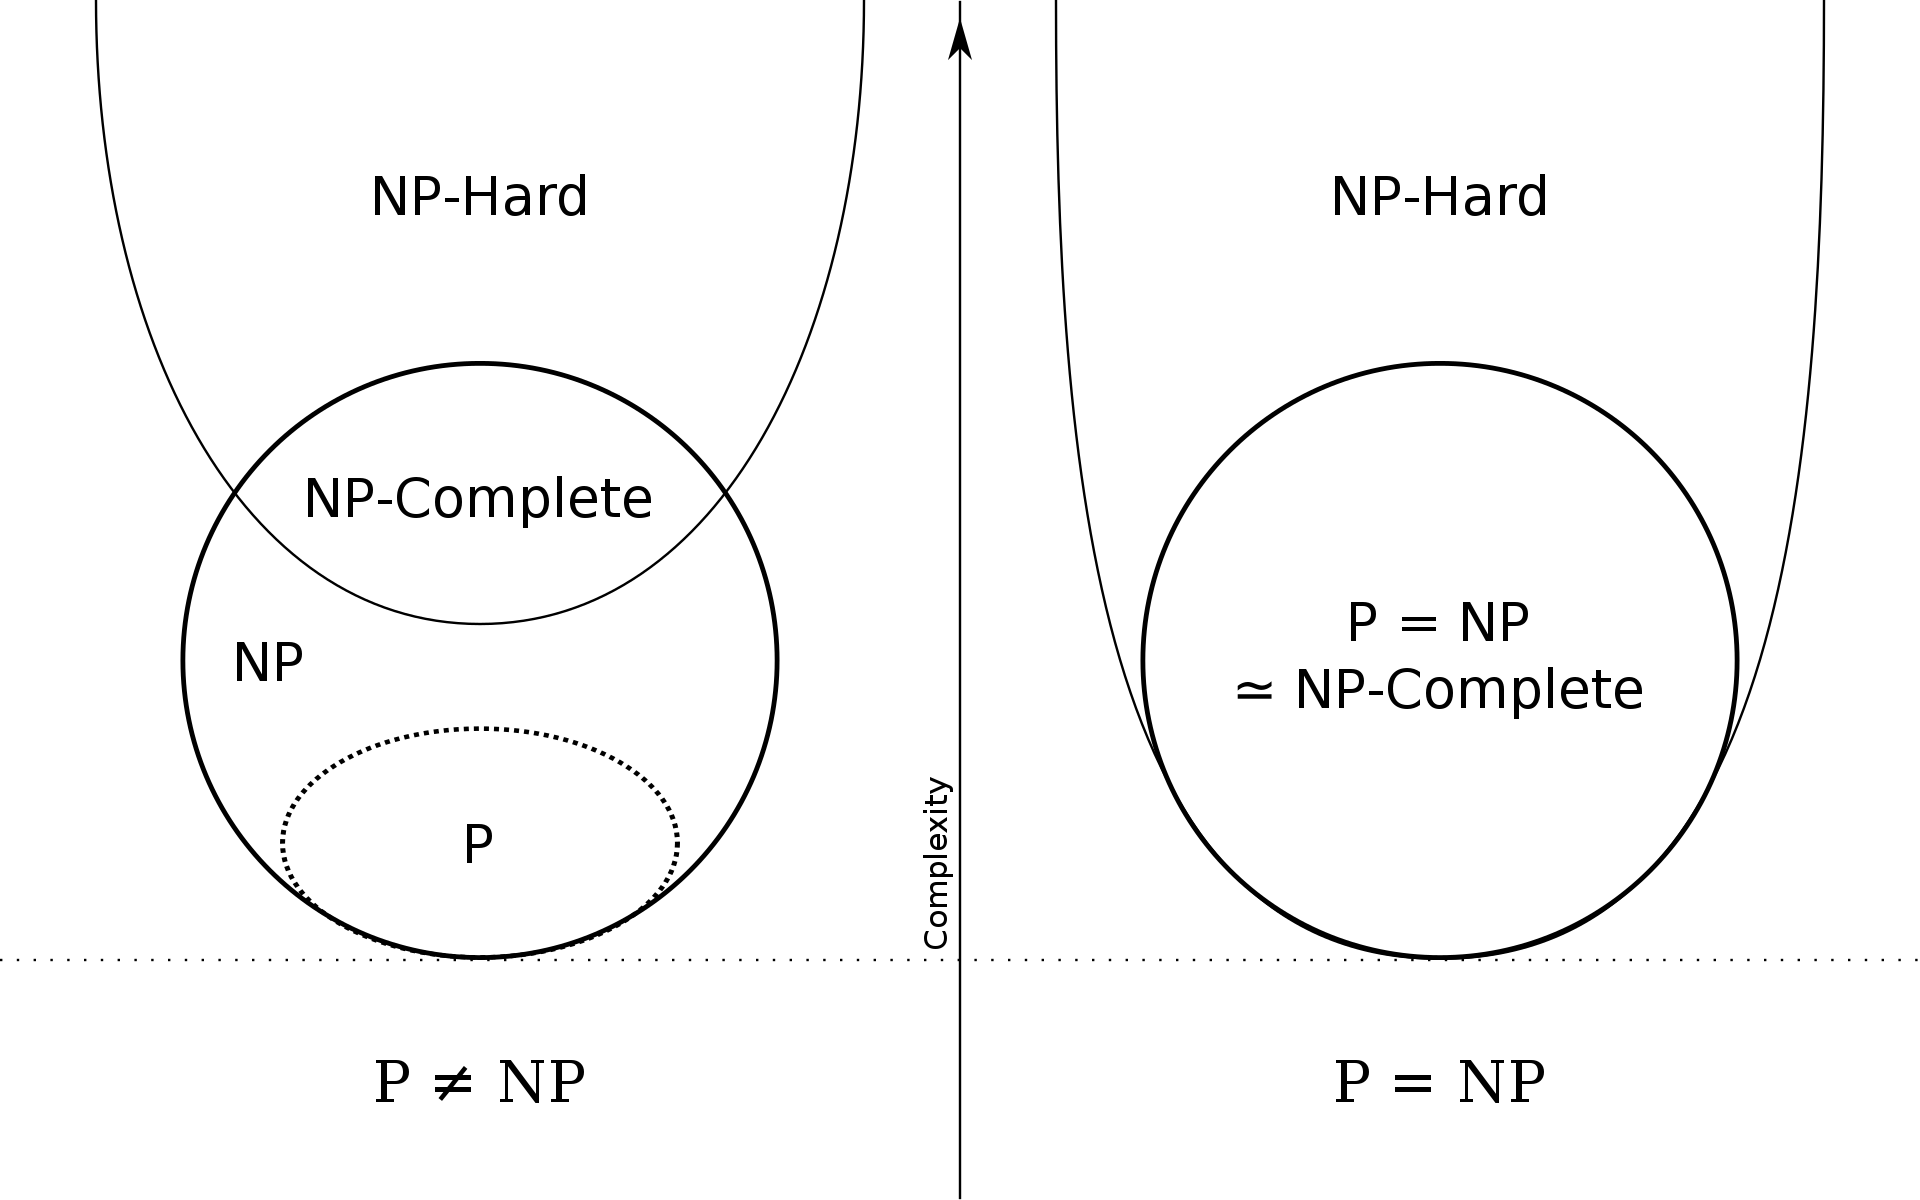
\includegraphics[width=1.\textwidth]{4}
    \caption{Взаимоотношение между классами P, NP, NP-complete (NP-полными задачами), NP-hard (NP-трудными задачами)}
    \label{fig:image1}
\end{figure}

Очевидно, что для доказательства NP полноты задачи необходимо доказать, что задача принадлежит классу NP и NP-hard.

Сначала нам нужно показать, что САМЫЙ ДЛИННЫЙ ПРОСТОЙ ЦИКЛ находится в NP. Экземпляр x представляет собой 
неориентированный граф и целое число k. Пусть сертификат y представляет собой последовательность не менее k 
вершин графа. Верификатор аналогичен верификатору для коммивояжера: он проходит по вершинам в сертификате одну 
за другой, помечая каждую из них на предмет отсутствия повторов и проверяя наличие ребра из каждой вершины в 
сертификате в вершину. следующий указанный в сертификате. Наконец, верификатор проверяет, что цикл завершается 
ребром из последней вершины в сертификате обратно в первую вершину. Если эти проверки удовлетворены, верификатор 
выводит 1. Если какие-либо из них не пройдены, верификатор выводит 0.

Этот верификатор занимает линейное время по количеству вершин. Если существует простой цикл, по крайней мере, с k 
вершинами, то передача этого цикла в качестве сертификата приводит к тому, что верификатор выводит 1. В противном 
случае ни один сертификат не содержит допустимого цикла, по крайней мере, с k вершинами, поэтому верификатор всегда
выводит 0 для этого экземпляра. Поскольку верификатор корректен и требует полиномиального времени, проблема в NP.

Чтобы показать, что задача является NP-трудной, мы сводим к ней HAM-CYCLE. Дан граф G, являющийся экземпляром HAM-ЦИКЛ,
определите экземпляр <G,k> САМОГО ДЛИННОГО ПРОСТОГО ЦИКЛА, содержащий тот же граф, и k=|V|, количество вершин в G.

Это сокращение включает в себя только простое копирование и подсчет, поэтому оно занимает полиномиальное время.

Теперь, если граф G содержит гамильтонов цикл, то этот цикл является простым циклом с |V| вершин, поэтому 
правильное решение для экземпляра САМЫЙ ДЛИННЫЙ ПРОСТОЙ ЦИКЛ равно 1. Если нет гамильтонова цикла, то нет простого
цикла с |V| или более вершин (просто по определению гамильтонова цикла), поэтому правильное решение для экземпляра
САМЫЙ ДЛИННЫЙ ПРОСТОЙ ЦИКЛ равно 0.

Итак, редукция верна и занимает полиномиальное время, показывая, что САМЫЙ ДЛИННЫЙ ПРОСТОЙ ЦИКЛ является NP-трудным.
Поскольку он также находится в NP, он является NP-полным.

\newpage
    
\begin{thebibliography}{3}
    \bibitem{1}
        Томас Кормен "Алгоритмы. Построение и анализ", 2005 год. Яз. рус.
    \end{thebibliography}

\end{document}